%%%%%%%%%%%%%%%%%%%%%%%%%%%%%%%%%%%%%%%%%
% Short Sectioned Assignment LaTeX Template Version 1.0 (5/5/12)
% This template has been downloaded from: http://www.LaTeXTemplates.com
% Original author:  Frits Wenneker (http://www.howtotex.com)
% License: CC BY-NC-SA 3.0 (http://creativecommons.org/licenses/by-nc-sa/3.0/)
%%%%%%%%%%%%%%%%%%%%%%%%%%%%%%%%%%%%%%%%%

%----------------------------------------------------------------------------------------
%	PACKAGES AND OTHER DOCUMENT CONFIGURATIONS
%----------------------------------------------------------------------------------------

\documentclass[paper=a4, fontsize=11pt]{scrartcl} % A4 paper and 11pt font size
% ---- Entrada y salida de texto -----

\usepackage[T1]{fontenc} % Use 8-bit encoding that has 256 glyphs
\usepackage[utf8]{inputenc}
%\usepackage[default]{sourcesanspro}
\usepackage{fourier} % Use the Adobe Utopia font for the document - comment this line to return to the LaTeX default
% ---- Idioma --------

\usepackage[spanish, es-tabla]{babel} % Selecciona el español para palabras introducidas automáticamente, p.ej. "septiembre" en la fecha y especifica que se use la palabra Tabla en vez de Cuadro

% ---- Code insertion ----
\usepackage{minted}
\usepackage[breakable]{tcolorbox} %Genera boxes, lo usamos para el codigo
\BeforeBeginEnvironment{minted}{\begin{tcolorbox}[breakable]}%
	\AfterEndEnvironment{minted}{\end{tcolorbox}}%
\BeforeBeginEnvironment{inputminted}{\begin{tcolorbox}[breakable]}%
	\AfterEndEnvironment{inputminted}{\end{tcolorbox}}%

\usepackage{xpatch} %permite abrir environments al ejecutar ciertos comandos

\xpretocmd{\inputminted}{\begin{tcolorbox}}{}{}%
	\xapptocmd{\inputminted}{\end{tcolorbox}}{}{}%

\setminted{
fontsize=\small,
breaklines,
breaksymbolleft=
}
% ---- Otros paquetes ----
\usepackage{dirtree}
\usepackage{vmargin}

\usepackage{url} % ,href} %para incluir URLs e hipervínculos dentro del texto (aunque hay que instalar href)
\usepackage{hyperref} % ,href} %para incluir URLs e hipervínculos dentro del texto (aunque hay que instalar href)
\hypersetup{
	colorlinks=true,
	linkcolor=blue,
	filecolor=magenta,      
	urlcolor=blue,
}

\usepackage{xcolor}
\definecolor{light-gray}{gray}{0.95}
\definecolor{alizarin}{rgb}{0.82, 0.1, 0.26}
\definecolor{nyellow}{rgb}{0.91, 0.656, 0.0}
%\definecolor{indigo}{rgb}{0.29, 0.0, 0.51}
%	\textcolor{red}{p}
%	\textcolor{orange}{r}
%	\textcolor{yellow}{a}
%	\textcolor{green}{c}
%	\textcolor{blue}{t}
%	\textcolor{indigo}{i}
%	\textcolor{violet}{c}
%	\textcolor{red}{a}
%	\textcolor{orange}{s}
%	\textcolor{yellow}{,}
%	\textcolor{green}{I}
%	\textcolor{blue}{S}
%	\textcolor{indigo}{E}

\usepackage{amsmath,amsfonts,amsthm} % Math packages
%\usepackage{graphics,graphicx, floatrow} %para incluir imágenes y notas en las imágenes
\usepackage{graphics,graphicx, float} %para incluir imágenes y colocarlas
\usepackage[export]{adjustbox}
\graphicspath{{imagenes/}}

% Para hacer tablas comlejas
%\usepackage{multirow}
%\usepackage{threeparttable}

%\usepackage{sectsty} % Allows customizing section commands
%\allsectionsfont{\centering \normalfont\scshape} % Make all sections centered, the default font and small caps

%Remove warnings
\usepackage{silence}
\WarningFilter{scrartcl}{Usage of package `fancyhdr'}

\usepackage{fancyhdr} % Custom headers and footers
\pagestyle{fancyplain} % Makes all pages in the document conform to the custom headers and footers
\fancyhead{} % No page header - if you want one, create it in the same way as the footers below
\fancyfoot[L]{} % Empty left footer
\fancyfoot[C]{} % Empty center footer
\fancyfoot[R]{\thepage} % Page numbering for right footer
\renewcommand{\headrulewidth}{0pt} % Remove header underlines
\renewcommand{\footrulewidth}{0pt} % Remove footer underlines
\setlength{\headheight}{13.6pt} % Customize the height of the header

\numberwithin{equation}{section} % Number equations within sections (i.e. 1.1, 1.2, 2.1, 2.2 instead of 1, 2, 3, 4)
\numberwithin{figure}{section} % Number figures within sections (i.e. 1.1, 1.2, 2.1, 2.2 instead of 1, 2, 3, 4)
\numberwithin{table}{section} % Number tables within sections (i.e. 1.1, 1.2, 2.1, 2.2 instead of 1, 2, 3, 4)

\setlength\parindent{0pt} % Removes all indentation from paragraphs - comment this line for an assignment with lots of text

\newcommand{\horrule}[1]{\rule{\linewidth}{#1}} % Create horizontal rule command with 1 argument of height

\setmarginsrb{2 cm}{1 cm}{2 cm}{2 cm}{1 cm}{1.5 cm}{1 cm}{1.5 cm} %Aumenta los márgenes

%----------------------------------------------------------------------------------------
%	TÍTULO Y DATOS DEL ALUMNO
%----------------------------------------------------------------------------------------

\title{Asignatura: Informática Gráfica\\
	Título: Prácticas  \hspace{0.05cm} }   

\author{Yeray López Ramírez	}                             

\renewcommand*\contentsname{hola}

\makeatletter
\let\thetitle\@title
\let\theauthor\@author
\let\thedate\@date
\makeatother

%----------------------------------------------------------------------------------------
% DOCUMENTO
%----------------------------------------------------------------------------------------

\begin{document}
\begin{titlepage}
	\centering
	%\textsc{\LARGE Universidad de Granada}\\[2.0 cm]    
	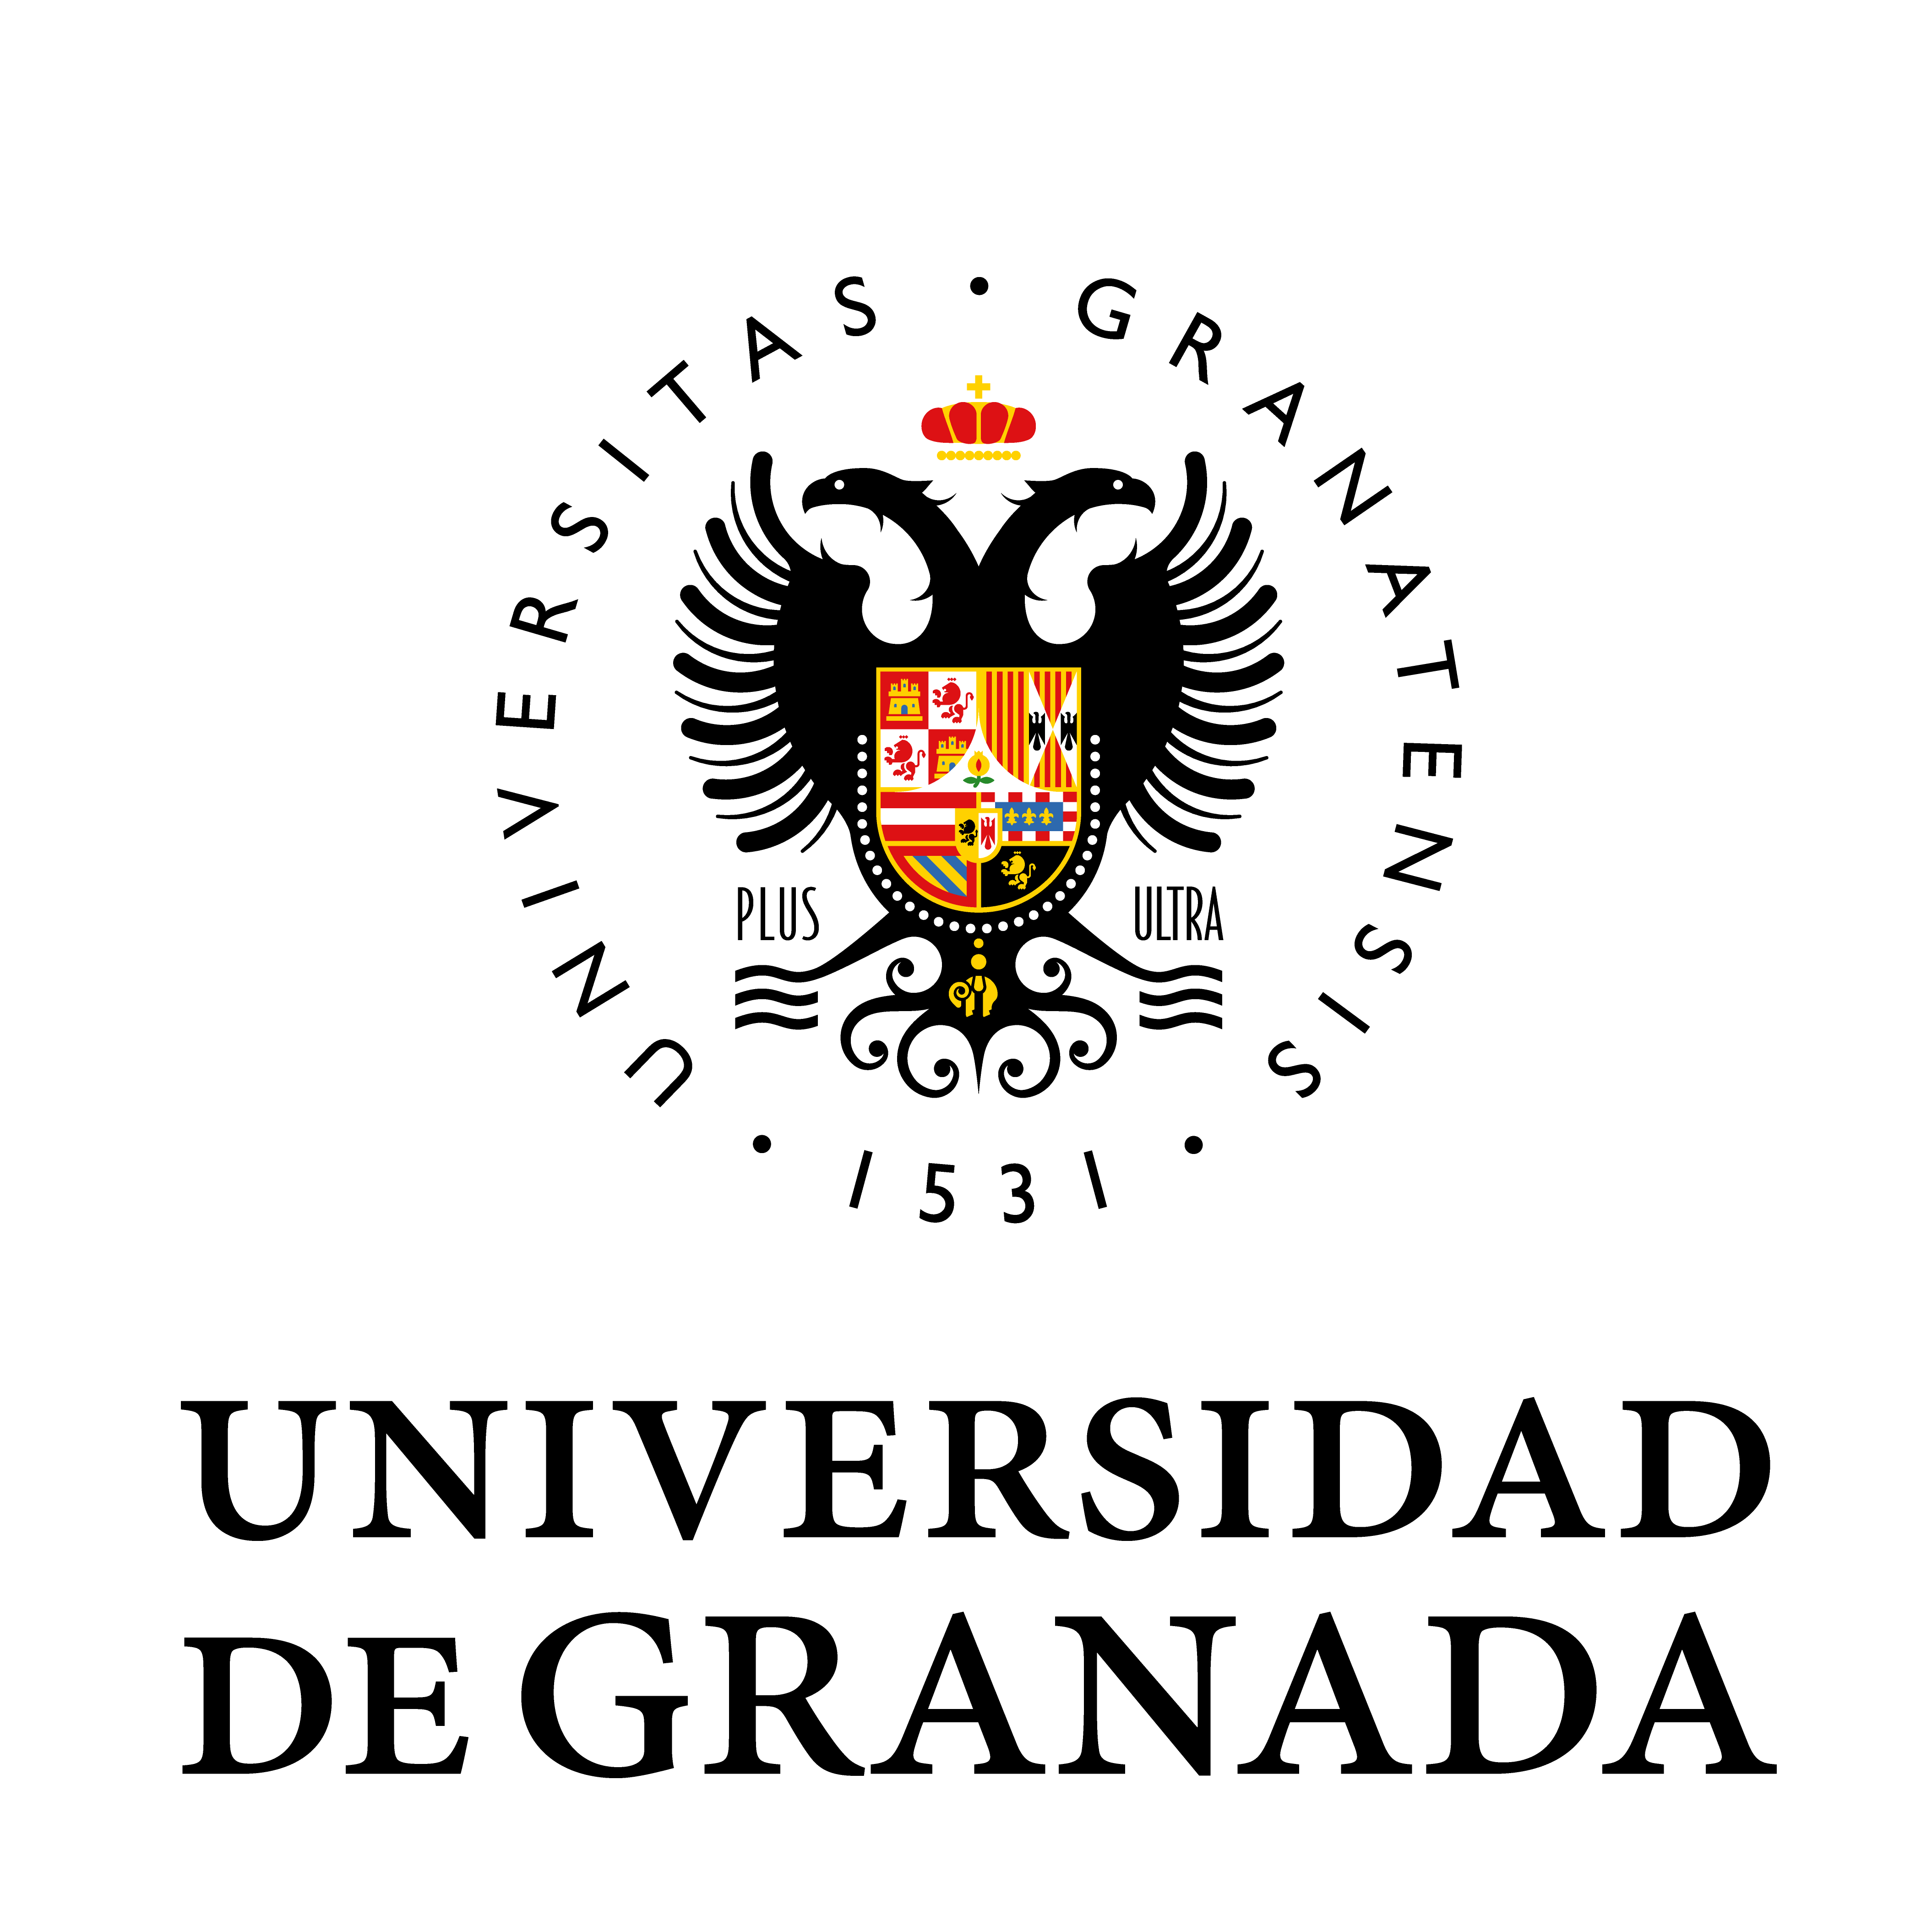
\includegraphics[scale = 0.6]{ugr.png}\\[1.0 cm]
	\rule{\linewidth}{0.2 mm} \\[0.4 cm]
	{ \huge \bfseries \thetitle}\\
	\rule{\linewidth}{0.2 mm} \\[1.5 cm]
	
	\begin{minipage}{0.5\textwidth}
		\begin{flushleft} \large
			\theauthor 
			123456789-Z \\
			\href{mailto:fulanito@correo.ugr.es}{fulanito@correo.ugr.es}
		\end{flushleft}
	\end{minipage}~
	\begin{minipage}{0.5\textwidth}
		\begin{flushright} \large
			Curso: 2022-23 \\
			Grupo A, 15:30 - 17:30 (Martes)                   
		\end{flushright}
	\end{minipage}\\[1 cm]
	
	{\small \thedate}\\[1 cm]
	
	\vfill
	
\end{titlepage}


\newpage %inserta un salto de página
\newcommand{\code}[1]{\colorbox{light-gray}{\textcolor{alizarin}{\texttt{#1}}}}
\newcommand{\high}[1]{\colorbox{light-gray}{\textcolor{nyellow}{\texttt{#1}}}}

\tableofcontents % para generar el índice de contenidos

\newpage

%----------------------------------------------------------------------------------------
%	Cuestión 1
%----------------------------------------------------------------------------------------

\section{Introducción}
A lo largo del curso he realizado 5 prácticas donde he aprendido a manejar opengl mediante código c++. Cada práctica se centra en un ámbito del diseño 3d y es lo que explicaré en esta breve memoria. Para facilitar el visualizado de las prácticas he creado un \code{switch-case} para cada práctica. Podemos cambiar entre prácticas con las teclas: \high{1},\high{2},\high{3},\high{4},\high{5}. Al final adjuntaré un listado con todas las teclas.
\section{Práctica 1}
Se accede con la tecla numérica: \code{1}\\
En esta primera práctica se ha diseñado figuras simples mediante la función \code{glVertex3f} y \code{glNormal3f} para las normales. También se utiliza \code{glColor3fv} y \code{glMaterial3fv} para el color y material de los objetos. He dibujado un cubo, una pirámide, un prisma pentagonal, un cono y un toroide. El resultado es:

\begin{figure}[H]
	\centering
	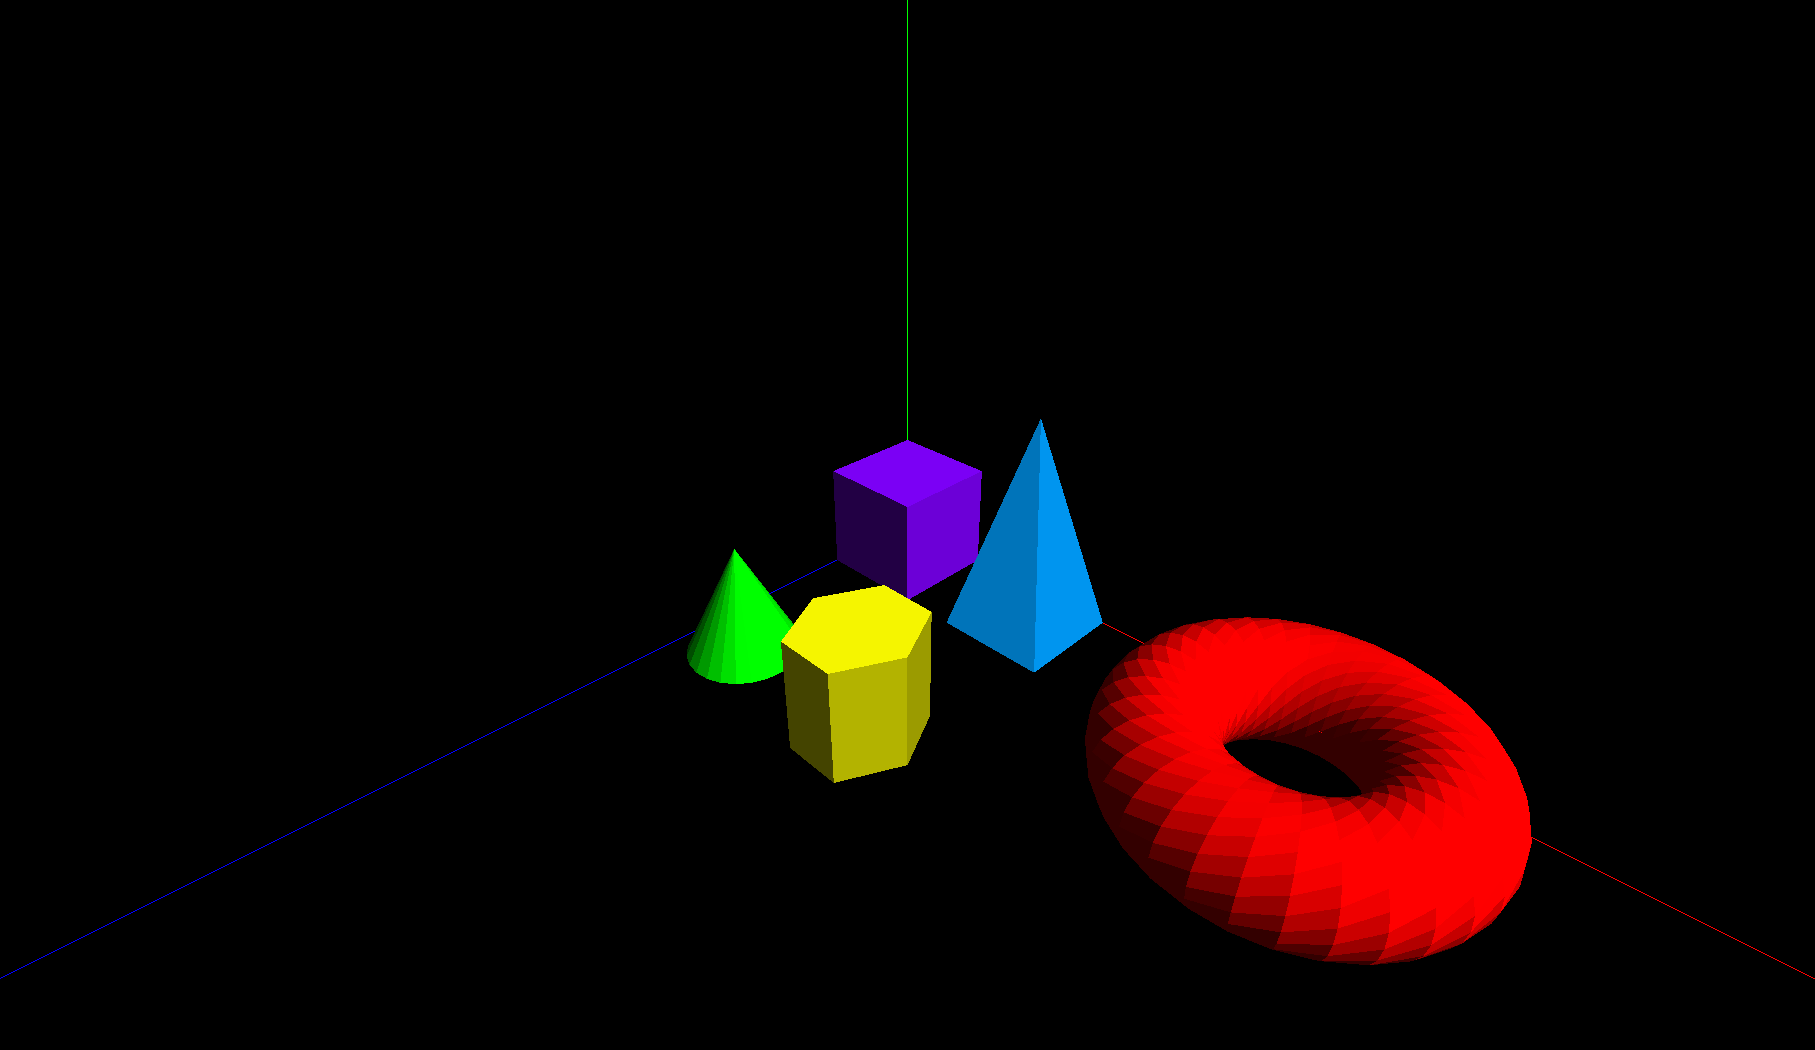
\includegraphics[width=1\linewidth]{figuras.png}
\end{figure} 

He creado un fichero para el cubo (cubo.c/h), otro para la pirámide (piramide.c/h) y otra para el prisma (prisma.c/h). El cono y el toroide son funciones de openGL. \\
Se modifica modelo.c añadiendo los draws de las figuras y se añaden las entradas de teclado a entradaTeclado.c

\section{Práctica 2}
Se accede con la tecla numérica: \code{2}\\
En esta segunda práctica se ha diseñado las clases de malla y objetoRevolucion para la lectura y visualización de objetos de malla y por revolución. También se calculan las normales con cálculo básico de vectores normales. Se dibuja a beethoven, un coche clásico, un peón y una fuente que es la figura diseñada a mano por mi. El resultado es:
\begin{figure}[H]
	\centering
	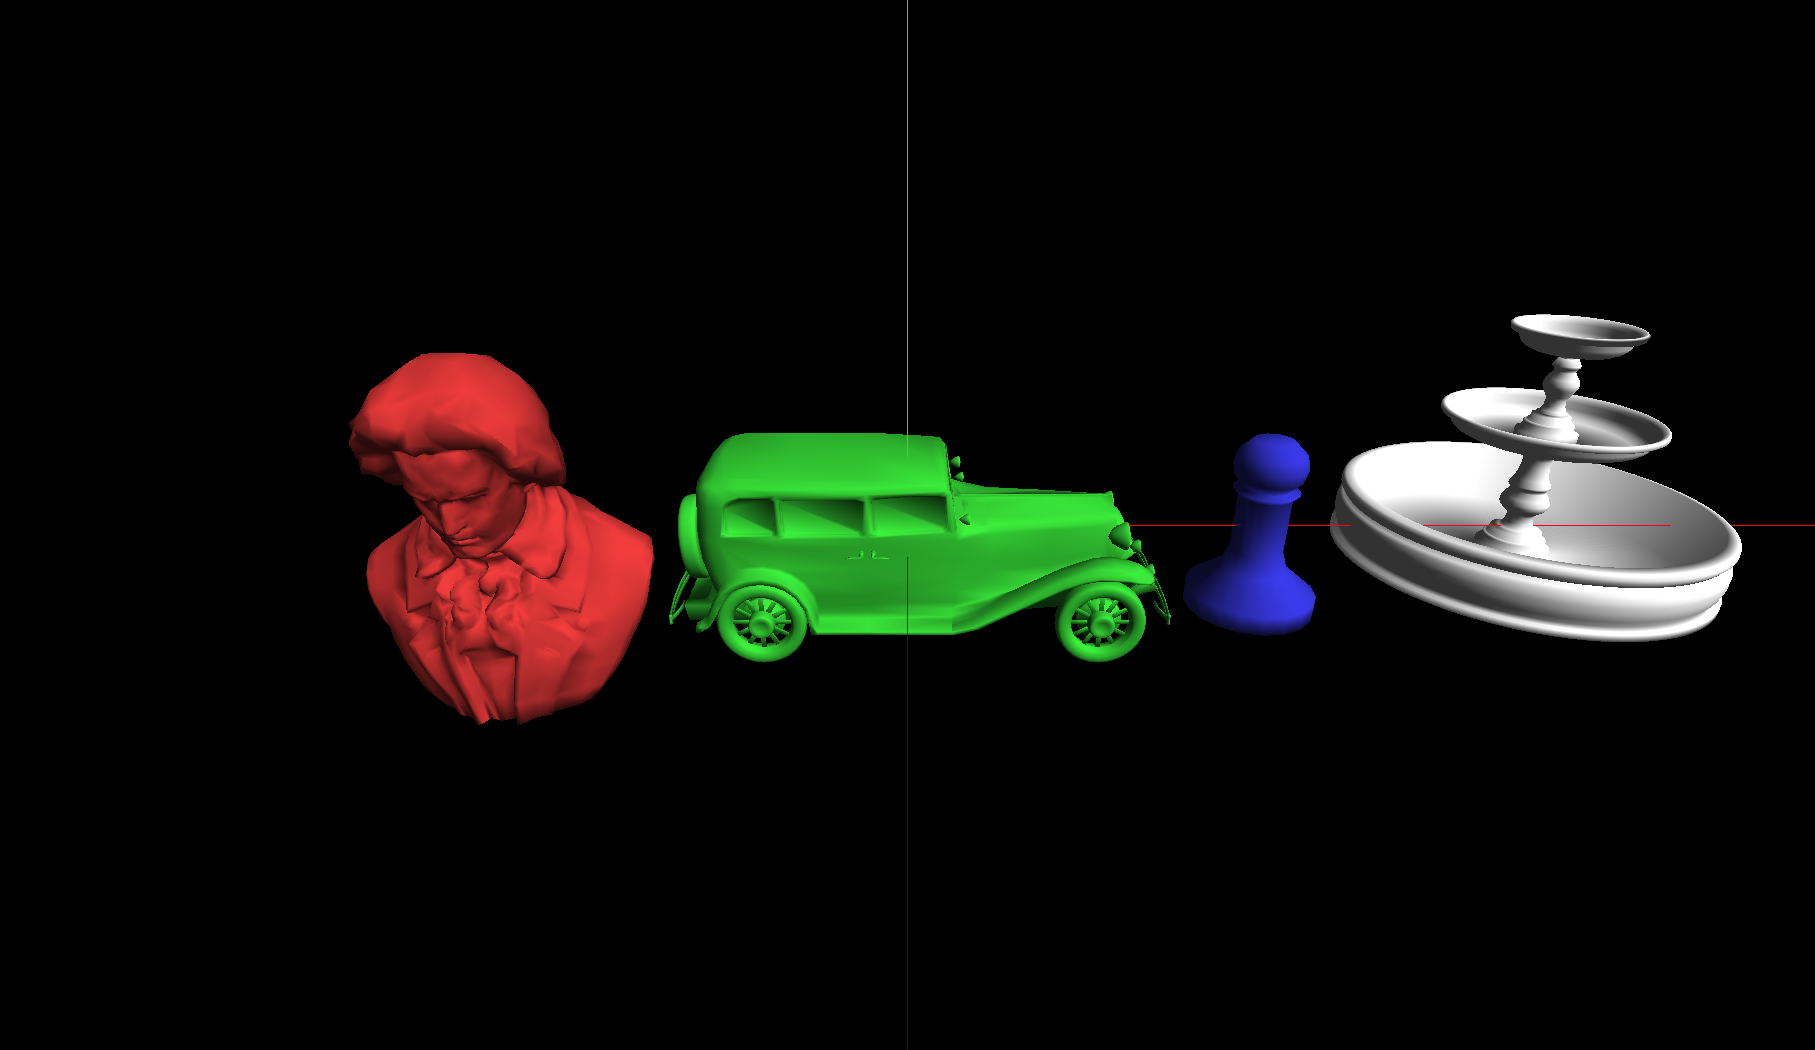
\includegraphics[width=1\linewidth]{figurasP2.png}
\end{figure} 

He creado los ficheros malla.c/h y objetoRevolucion.c/h para cada clase. 

\section{Práctica 3}
Se accede con la tecla numérica: \code{3}\\
En esta tercera práctica se ha diseñado un objeto jerárquico de 3 grados de libertad, en mi caso, una bicicleta. Está diseñada completamente a base de cilindros (el cuerpo, las llantas, las cadenas, los piñones), ortoedros (pedales),  objetos de revolución para las ruedas y un objeto ply para el sillín. Puede moverse hacia delante/atrás, pedalear en ambos sentidos, ajustar el sillín arriba o abajo y mover las ruedas en sentido horario y antihorario. El resultado es:
\begin{figure}[H]
	\centering
	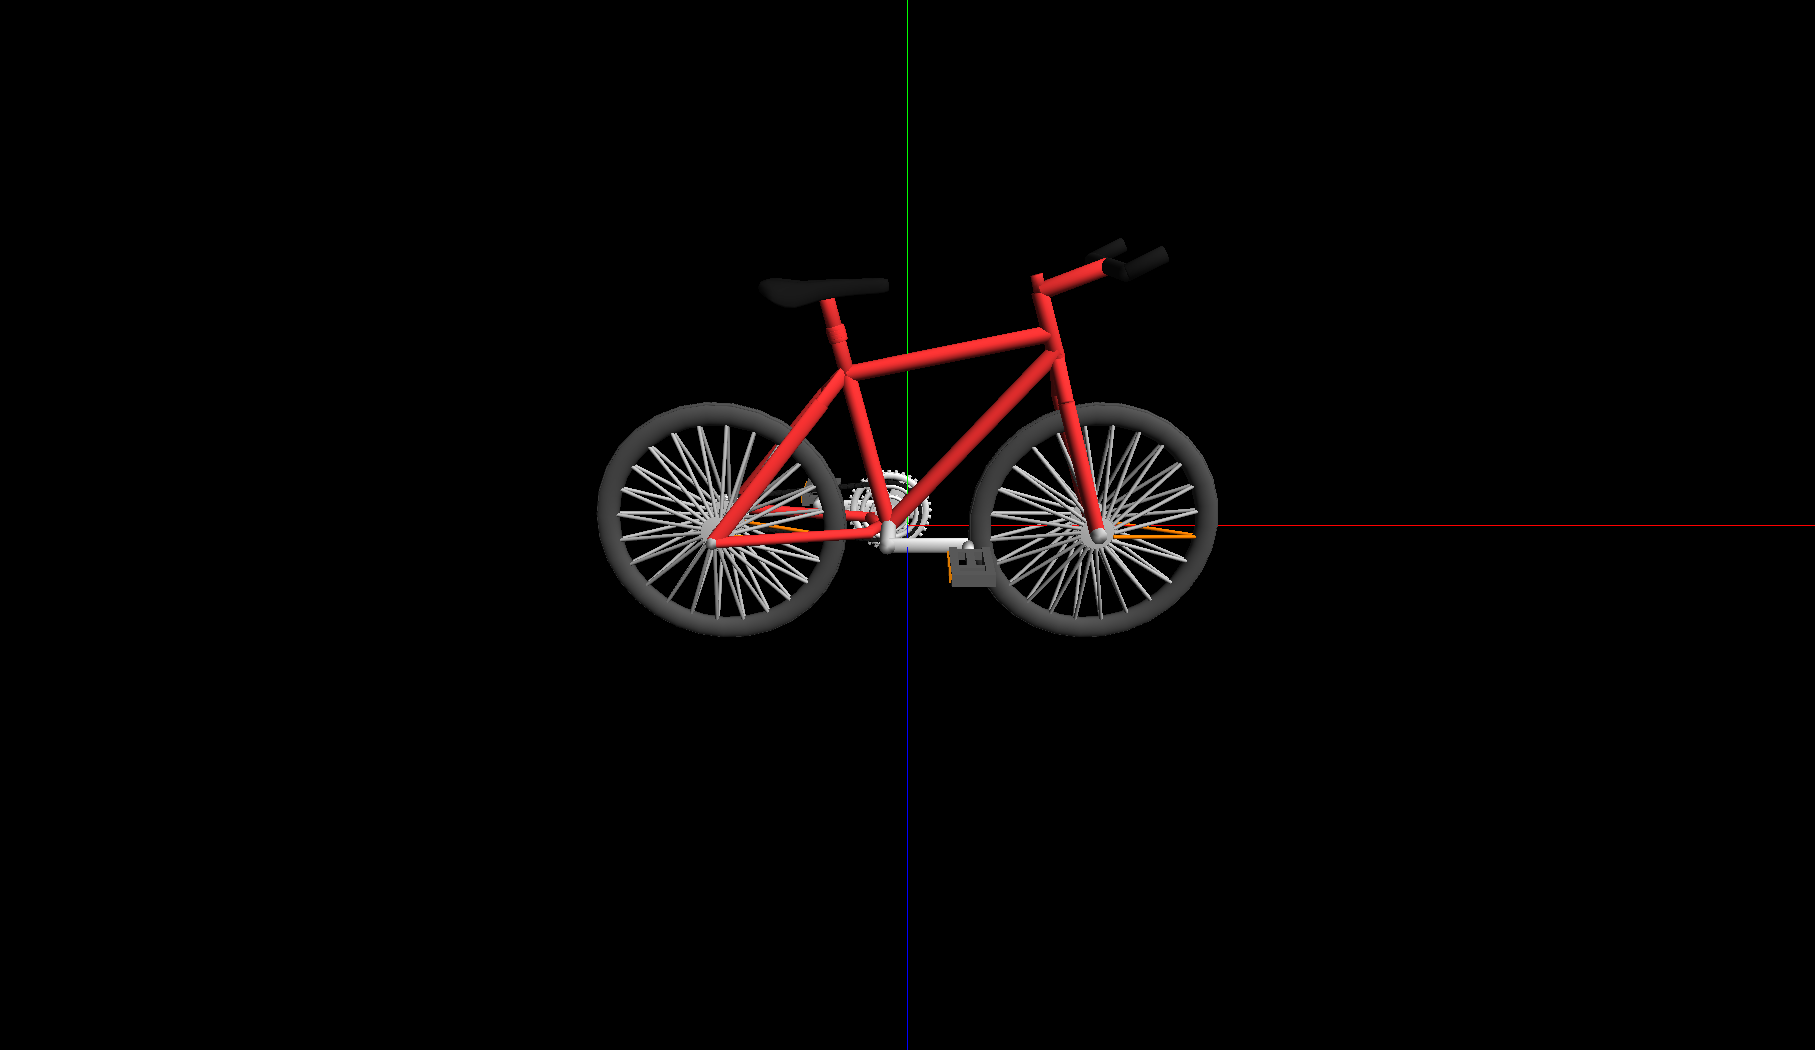
\includegraphics[width=1\linewidth]{figurasP3.png}
\end{figure} 

He creado un fichero bici.c/h para implementar todas las funcionalidades de la bicicleta.

\section{Práctica 4}
Se accede con la tecla numérica: \code{4}\\
En esta cuarta práctica se han añadido nuevos materiales y texturas a las mallas y objetos de revolución. Se dibujan 3 peones de distinto material: el primero es negro macizo, el segundo es rojo reflectante y el tercero verde brillante. Además de un dado (un cubo con textura de dado) y una lata de cerveza con tapas texturizadas debidamente. El resultado es:
\begin{figure}[H]
	\centering
	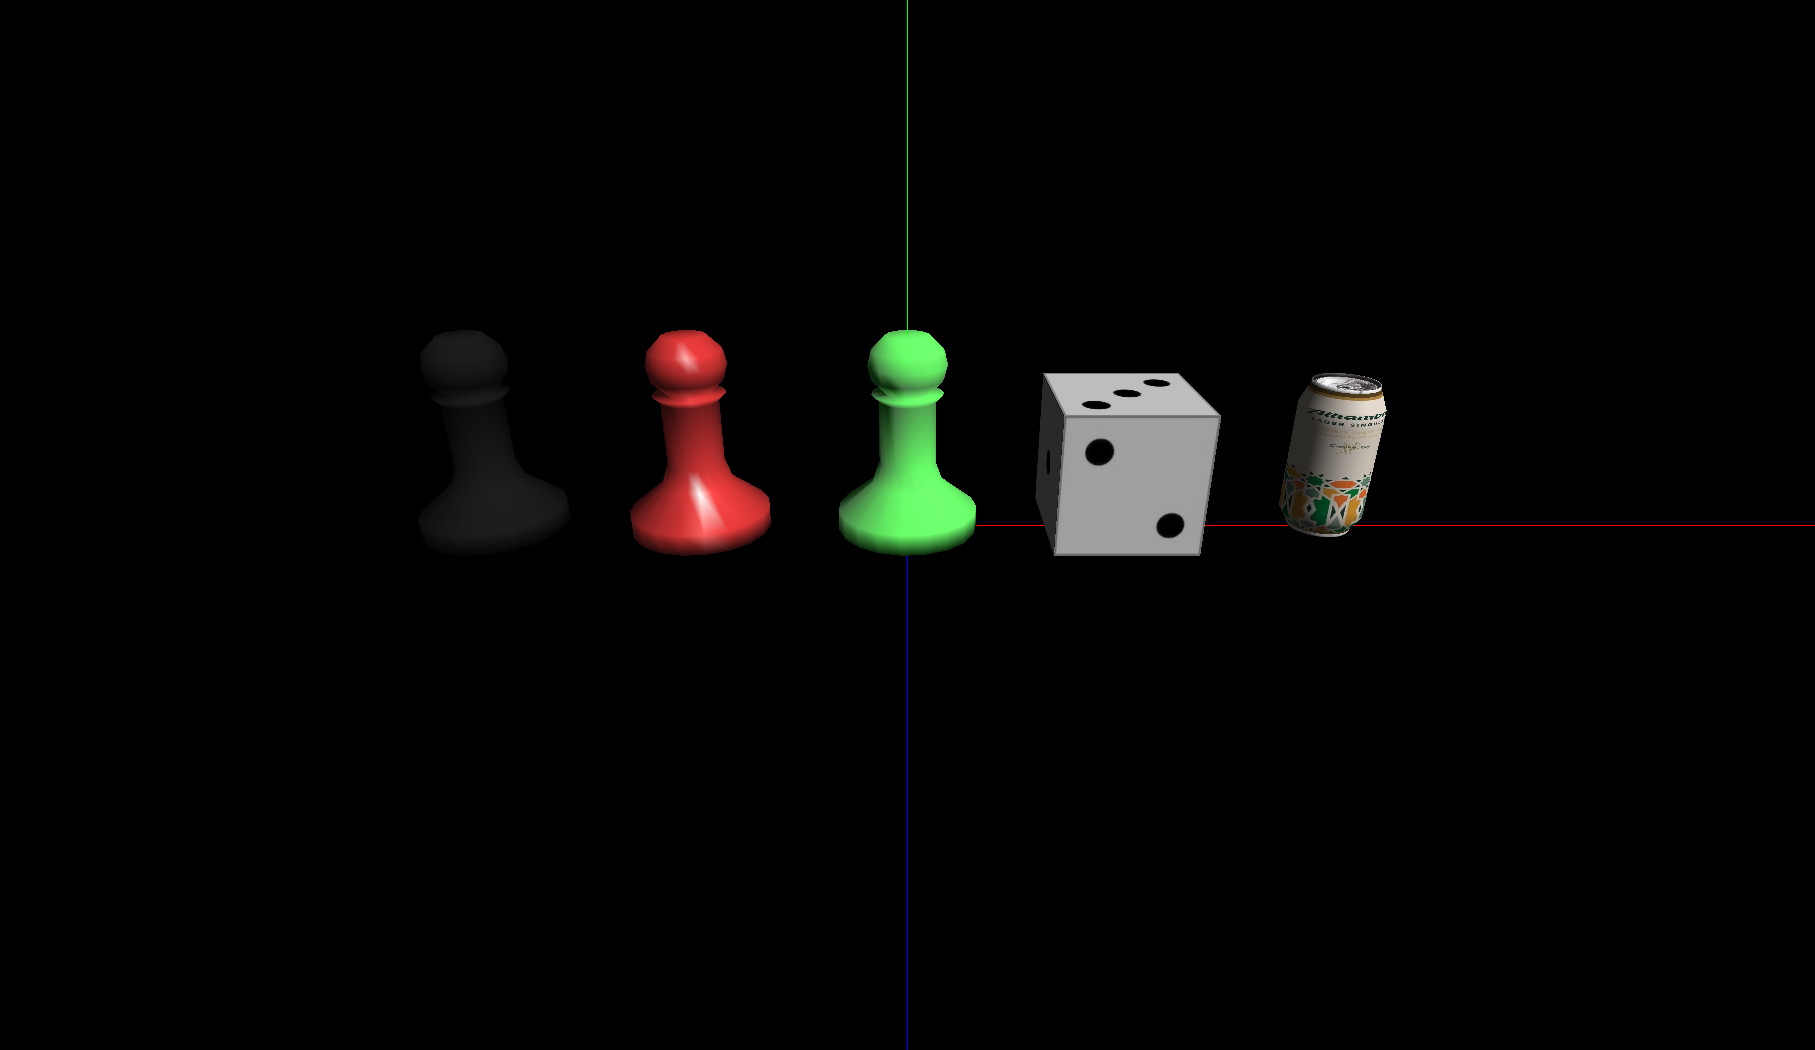
\includegraphics[width=1\linewidth]{figurasP4.png}
\end{figure} 

Se modifican las clases malla.c y objetosRevolucion.c añadiendo constructores y funciones de textura. Para los materiales se añade una función setMateriales en las mallas.

\section{Práctica 5}
Se accede con la tecla numérica: \code{5}\\
En esta quinta práctica se ha manipulado la cámara para implementar las vistas perspectiva y ortogonal y sus respectivas representaciones: alzado, planta y perfil. También se ha modificado la cámara para que pueda moverse por el escenario con el teclado y gestionar la rotación con el ratón. Por último se ha implementado la selección de figuras con el color magenta y un pequeño menú de glut para modificar el color de las figuras seleccionadas. Se dispone de varios colores por defecto: blanco, celeste, naranja, rojo, verde y azul. Se dibujan las figuras de la práctica 2,3 y 4. El resultado es:

\begin{figure}[H]
	\centering
	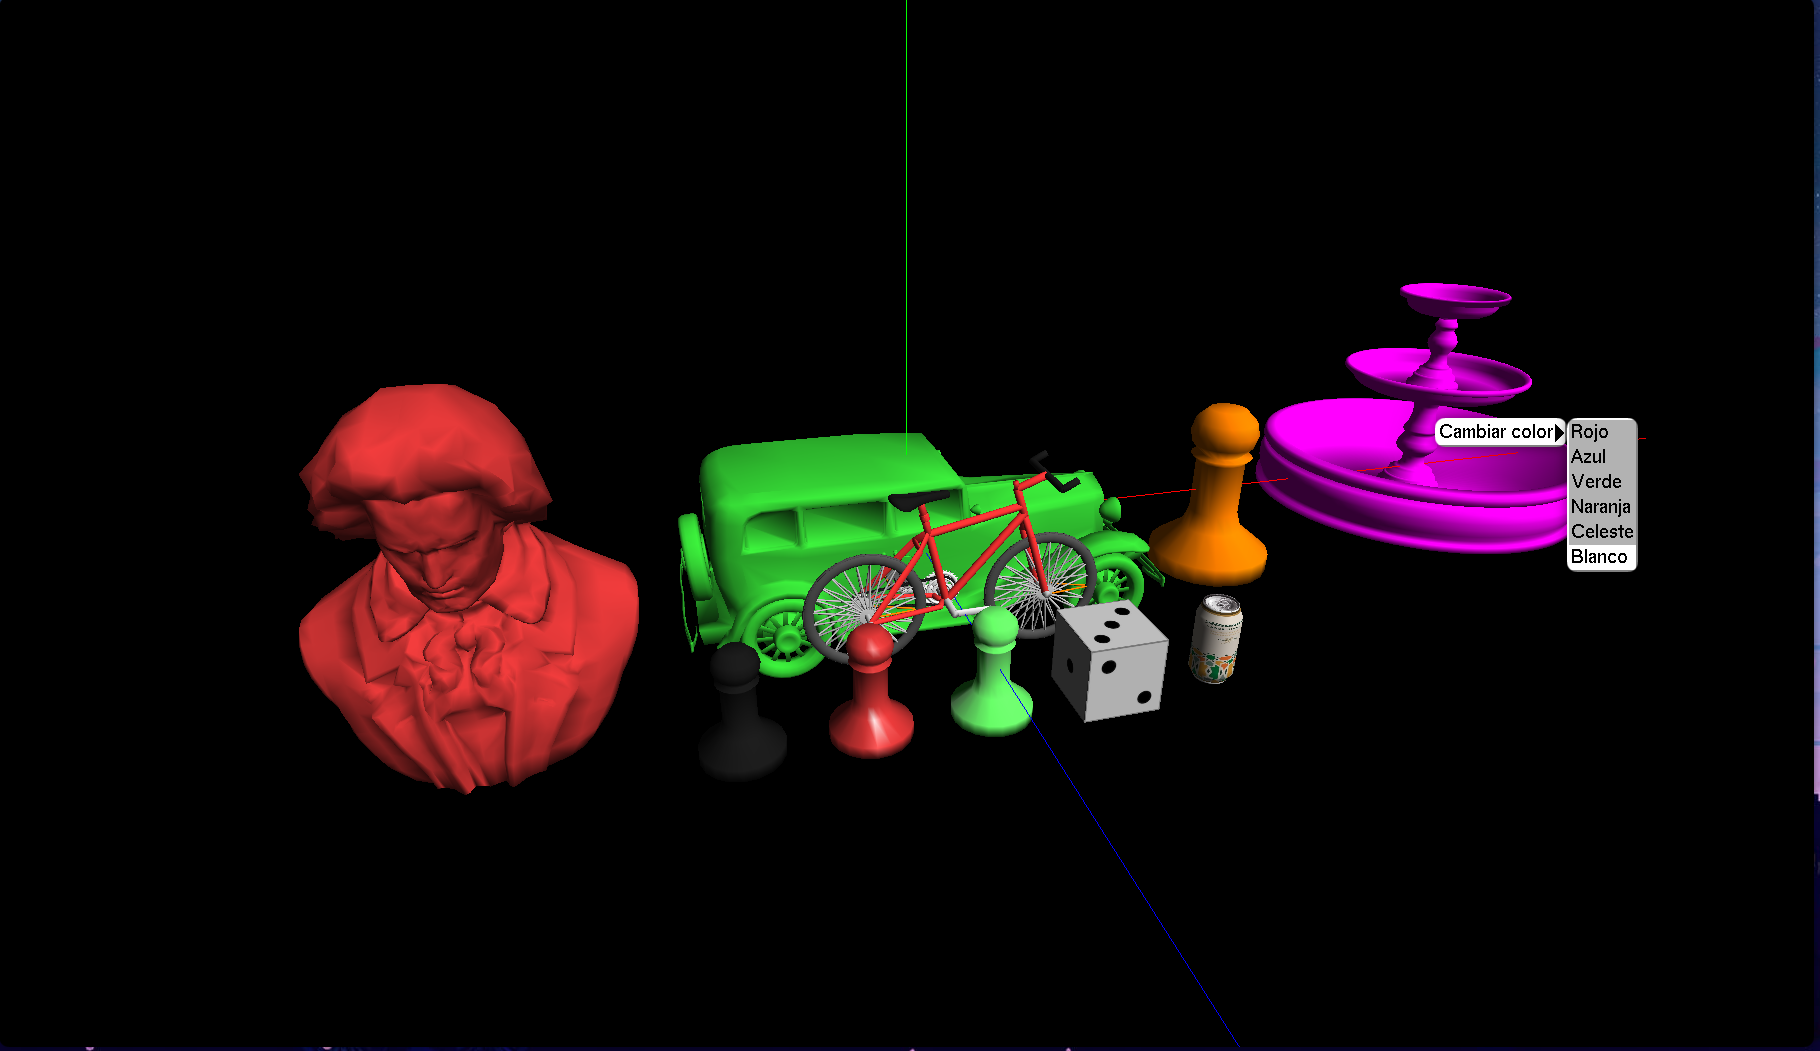
\includegraphics[width=1\linewidth]{figurasP5.png}
\end{figure} 

Se modifican los ficheros raton.c para mover la cámara con el ratón, visual.c y entradaTeclado.c para el menú y las vistas y por último malla.c y modelo.c para para la selección de figuras.

\section{Listado de teclas}
A continuación se listan todas las teclas y su función:
\begin{enumerate}
	\item Para cambiar de practicas:
	\begin{itemize}
		\item \code{1}: Practica 1
		\item \code{2}: Practica 2
		\item \code{3}: Practica 3
		\item \code{4}: Practica 4
		\item \code{5}: Practica 5
	\end{itemize}
	\item \code{p}: Modo punto (muestra los puntos de las figuras)
	\item \code{l}: Modo linea (muestra las lineas de las figuras)
	\item \code{f}: Modo relleno (muestra el relleno de las figuras)
	\item \code{i}: Activar/Desactivar iluminación
	\item \code{y}: Modo caras o vértices
	\item Animación de la bicicleta:
	\begin{itemize}
		\item \code{u}: Activar/Desactivar animación
		\item \code{E/e}: Avanzar o retroceder bici
		\item \code{T/t}: Subir o bajar el asiento
		\item \code{O/o}: pedalear hacia delante/atrás
		\item \code{N/n}: girar ruedas en sentido del reloj/contrarreloj
		\item \code{f}: Velocidad x1
		\item \code{g}: Velocidad x2
		\item \code{h}: Velocidad x2.5
		\item \code{j}: Velocidad x2.75
		\item \code{k}: Velocidad x3
	\end{itemize}
	\item \code{c}: Alternar luz 1/2 (blanca/roja)
	\item \code{f1}: vista perfil (ortogonal)
	\item \code{f2}: vista alzado (perspectiva)
	\item \code{f3}: vista planta (perspectiva)
	\item \code{f4}: alternar vista perspectiva/ortogonal
	\item \code{r}: Reinicia la vista a una posición por defecto (0 de rotación y 10 de distancia)
	\item \code{a}: Desplaza la cámara -x
	\item \code{d}: Desplaza la cámara +x
	\item \code{w}: Desplaza la cámara -z
	\item \code{s}: Desplaza la cámara +z
	\item \code{Click izquierdo}: selecciona la figura. Mueve la cámara si se mantiene pulsado y se arrastra.
	\item \code{Arrastrar con click medio}: rota la cámara acorde al movimiento del ratón
	\item \code{Click derecho}: abre el menú de selección de color del material
\end{enumerate}

\end{document}
